\chapter{Funcionalidades do MDArte}
Neste capítulo iremos explorar algumas funcionalidades que já existem no MDArte,
a fim de agilizar e simplificar o processo de desenvolvimento. Para tal
alteraremos os modelos de \texttt{CRUD} gerados automaticamente pelo
\texttt{MDArte}. Para evitar que as alterações feitas sejam sobrescritas por
engano, vá no diagrama de classe que descreve as entidades do Banco de Dados,
abra a especificação da classe \texttt{Estudante}, selecione a aba
\texttt{stereotypes} e remova o estereótipo \texttt{«Manageable»}.

\section{Campo com Autocomplete}
Nesta seção veremos como implementar um \texttt{autocomplete} para um
determinado campo de texto. Iremos transformar o campo \texttt{matricula} do
caso de uso \texttt{Consulta Estudante} em um campo com \texttt{autocomplete}.

O modelo inicial do caso de uso \texttt{Consulta Estudante} no  \texttt{CRUD}
para a entidade estudante pode ser visto na imagem \ref{modelo_consulta_estudante}:
\begin{figure}[H]
	\centering
	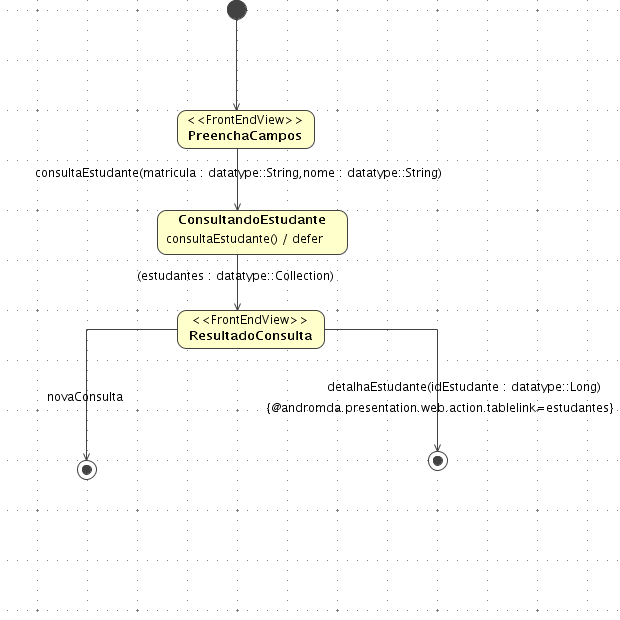
\includegraphics[width=350pt,height=300pt]{files/imgs/tutorial-mdarte-0028.png}
	\caption{Modelo do caso de uso Consulta Estudante.}
	\label{modelo_consulta_estudante}
\end{figure}

Abriremos a especificação da \texttt{transition} que sai da \texttt{front end
view} de nome \texttt{preencha os campos}, clicaremos no botão \texttt{edit}, no
\texttt{fieldset} \texttt{trigger}. Na aba \texttt{parameters}, da janela
\texttt{signal event specification}, que será aberta automaticamente, dê duplo
clique no nome do parâmetro \texttt{matricula} e será então aberta a
especificação do parâmetro. Selecione então a aba \texttt{tagged values},
selecione o \texttt{tagged value}
\texttt{@andromda.presentation.web.view.field.type} e clique no botão
\texttt{create value}. Selecione então a opção \texttt{autocomplete}, como na
imagem \ref{field_type_autocomplete}.
\begin{figure}[H]
	\centering
	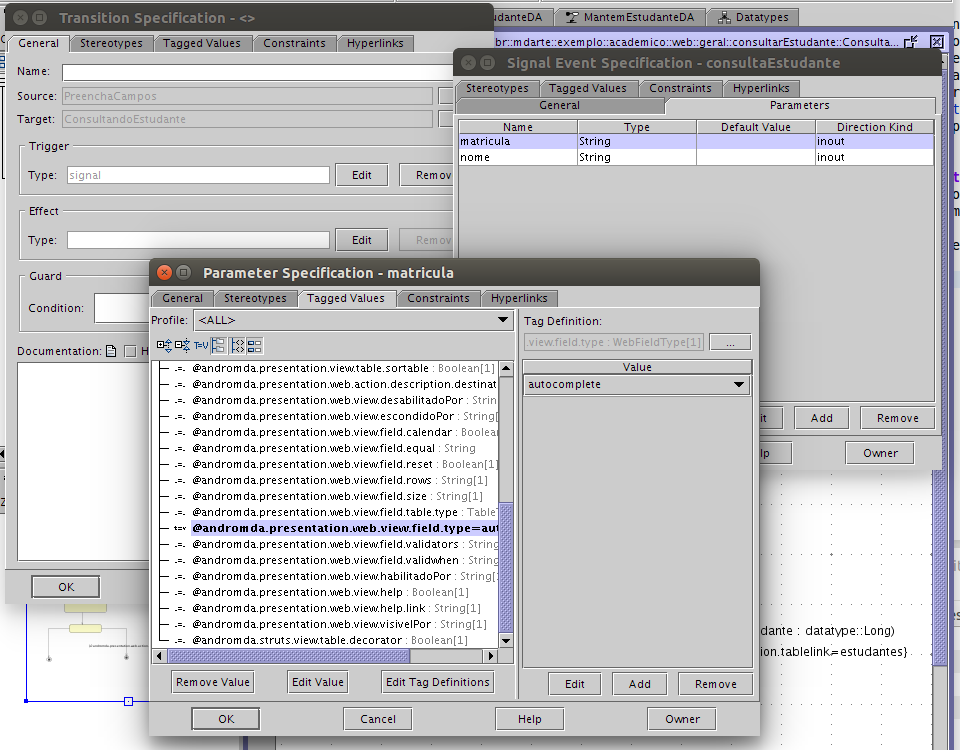
\includegraphics[width=350pt,height=300pt]{files/imgs/tutorial-mdarte-0027.png}
	\caption{Adicionando o field type 'autocomplete' à um campo da view.}
	\label{field_type_autocomplete}
\end{figure}

Agora executaremos o seguinte comando no terminal na raiz do projeto:
\begin{lstlisting}[language=bash]
maven mda -Dprojeto=sistemaacademico-geral-Estudante
\end{lstlisting}

Feito isto, o \texttt{MDArte} gerará automaticamente toda a estrutura
responsável por receber e tratar as requisições assíncronas para o preenchimento do
\texttt{autocomplete}, restando ao desenvolver apenas implementar no
\texttt{ControleImpl} a filtragem dos valores retornados, de acordo com o valor
do campo. Para isto, criaremos, na classe
\texttt{ConsultaEstudanteControleImpl}, um método seguindo o seguinte padrão 
\texttt{protected String[]
<nome-do-campo><nome-do-caso-de-uso>AutoComplete(java.lang.String query,
org.andromda.bpm4struts.ViewContainer container)}. Vejamos abaixo um exemplo de
implementação para o \texttt{autocomplete} do nosso campo de \texttt{matrícula}:

\begin{framed}
\lstinputlisting[language=java]{files/java/autocomplete.java}
\end{framed}

Agora executaremos o seguinte comando para compilar e dar \texttt{deploy} no
\texttt{Sistema Acadêmico} :
\begin{lstlisting}[language=bash]
maven compile deploy
\end{lstlisting}

Feito isto, daremos \texttt{start} no \texttt{JBoss} e abriremos o sistema e
faremos login. Na tela \texttt{Preencha os Campos} do caso de uso
\texttt{Consulta Estudante} podemos agora verificar o \texttt{autocomplete}
funcionando, como na imagem \ref{exemplo_autocomplete}.
\begin{figure}[H]
	\centering
	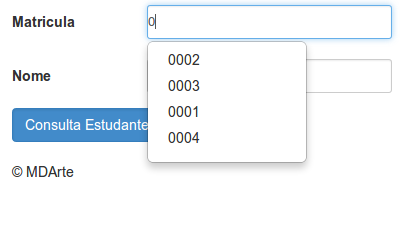
\includegraphics[width=350pt,height=300pt]{files/imgs/tutorial-mdarte-0029.png}
	\caption{Exemplo de autocomplete.}
	\label{exemplo_autocomplete}
\end{figure}

\section{Tabela assíncrona (JTable)}
Nesta seção veremos como implementar uma tabela \texttt{assíncrona}
(\texttt{JTable}) usando o \texttt{MDArte}. Para tal, vamos considerar como
ponto de partida o modelo do caso de uso \texttt{Consulta Estudante} conforme as
alterações feitas no tópico anterior. Certifique-se de ter removido o
estereótipo \texttt{«Manageable»} da classe \texttt{Estudante} no diagrama de
classes que descreve a \texttt{Camada de domínio}, a fim de evitar que o
\texttt{CRUD} seja re-gerado, sobrescrevendo assim as alterações que faremos.

Veremos agora, por subseções, algumas das funcionalidades disponíveis na tabela
assíncrona.

\subsection{Implementando uma tabela simples}
Para implementar uma tabela assíncrona, precisamos primeiramente abrir o modelo
do caso de uso \texttt{Consulta Estudante}, abriremos então a especificação da
\texttt{transition} que sai da \texttt{action} \texttt{ConsultandoEstudante}
para \texttt{Front End View} \texttt{'ResultadoConsulta'}, clicar no botão
\texttt{edit} no \texttt{fieldset} \texttt{trigger}, iremos então na aba
\texttt{parameters}, na janela \texttt{signal event specification}, aberta
automaticamente. Daremos então um duplo clique no nome do parâmetro
(\texttt{estudantes}), que representa a tabela que será mostrada na view.
Selecionaremos a aba \texttt{tagged values} selecione o \texttt{tagged value}
\texttt{@andromda.presentation.web.view.field.table.type} e clique no botão
\texttt{create value}. Selecione então a opção \texttt{jtable}, como na
imagem \ref{table_type_jtable}.
\begin{figure}[H]
	\centering
	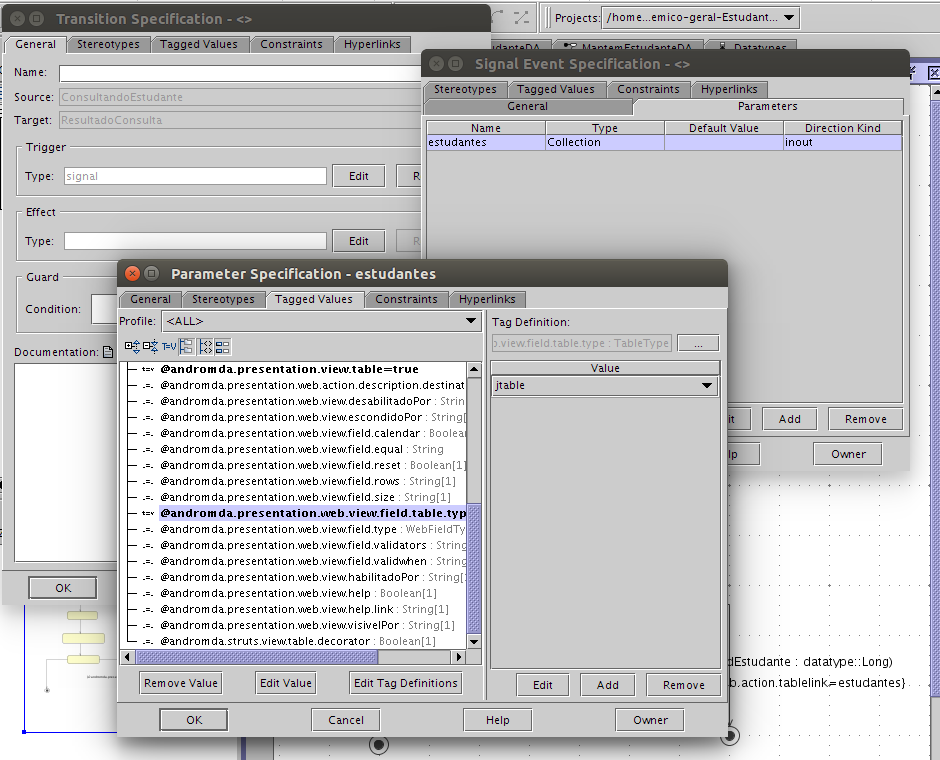
\includegraphics[width=350pt,height=300pt]{files/imgs/tutorial-mdarte-0030.png}
	\caption{Mudando tipo da tabela para 'jtable'.}
	\label{table_type_jtable}
\end{figure}

Agora executaremos o seguinte comando no terminal na raiz do projeto:
\begin{lstlisting}[language=bash]
maven mda -Dprojeto=sistemaacademico-geral-Estudante
\end{lstlisting}

Feito isto, o MDArte já terá gerado toda a estrutura necessária pela recepção e
tratamento das requisições assíncronas da tabela, restando ao desenvolvedor
implementar somente dois métodos: um para indicar o numero total de elementos a
serem exibidos na tabela, usado para fazer a paginação da mesma, e outro para
retornar a coleção de objetos a serem exibidos na página atual da tabela.

A assinatura do método para o carregamento da tabela segue o seguinte padrão:

\begin{lstlisting}[language=java]
protected Collection load[nome-da-view][nome-da-tabela]Table(Integer paginacao,
Integer linhas, String propriedade, Boolean desc, ViewContainer container) 
\end{lstlisting}

A assinatura do método que retorna o total de elementos na tabela segue o
seguinte padrão:

\begin{lstlisting}[language=java]
protected Integer get[nome-da-view][nome-da-tabela]TableLength(Integer
paginacao, Integer linhas, String propriedade, Boolean desc, ViewContainer
container) throws Exception
\end{lstlisting}

Também será necessário alterar o método \texttt{carregaDados} do
\texttt{ControllerImpl} para disponibilizar as informações preenchidas na
\texttt{PreenchaCampos} para serem usadas pela tabela disponível na
\texttt{view} \texttt{ResultadoConsulta}.

Abaixo o exemplo de implementação para a tabela \texttt{estudantes} da
\texttt{view ResultadoConsulta} no caso de uso \texttt{Consulta Estudante}.

\begin{framed}
\lstinputlisting[language=java]{files/java/JTableSimples.java}
\end{framed}

Não se esqueça de fazer os \texttt{imports} necessários de acordo com as
alterações feitas. Se o seu \texttt{.classpath} estiver corretamente
configurado, você pode usar o atalho \texttt{Ctrl + Shift + O}, do eclipse, que
importará automaticamente todas as classes que estão faltando.

Agora, compilaremos e daremos deploy do código da aplicação, com o seguinte
comando:
\begin{lstlisting}[language=bash]
maven compile deploy
\end{lstlisting}

Abriremos agora a view \texttt{PreenchaCampos} e digitaremos um valor para
filtragem dos dados da entidade \texttt{Estudante}. Como na imagem
\ref{preencha_campos_tabela_async_simples}.
\begin{figure}[H]
	\centering
	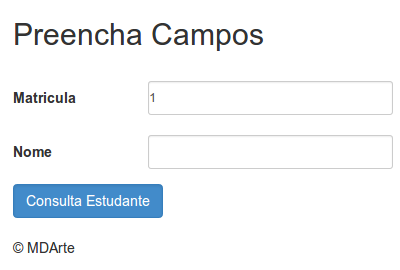
\includegraphics[width=260pt,height=180pt]{files/imgs/tutorial-mdarte-0031.png}
	\caption{Filtrando dados da tabela assíncrona de Estudantes.}
	\label{preencha_campos_tabela_async_simples}
\end{figure}

Na imagem \ref{resultado_consulta_tabela_async_simples}, podemos ver a tabela
carregada com os dados resultantes da filtragens. 
\begin{figure}[H]
	\centering
	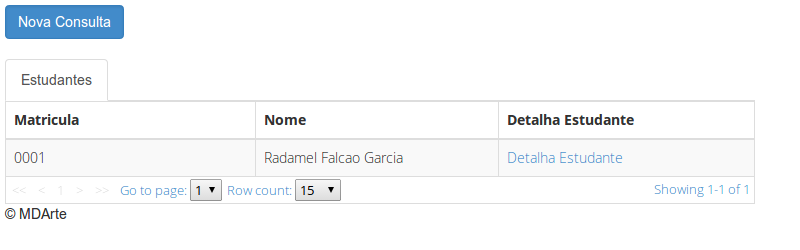
\includegraphics[width=460pt,height=200pt]{files/imgs/tutorial-mdarte-0032.png}
	\caption{Filtragem dos dados da tabela assíncrona de Estudantes.}
	\label{resultado_consulta_tabela_async_simples}
\end{figure}

Note que o funcionamento da tabela se dá por requisições assíncronas
ao servidor, acabando com a necessidade de recarregar a página para alterar seus
dados. 

O \texttt{MDArte} já dá suporte a diversos tipos de chamadas assíncronas que se
possa querer fazer fazer com a tabela, no entanto, caso haja a necessidade de
mais informações sobre o funcionamento da mesma, a documentação pode ser
acessada \href{http://www.jtable.org/Home/Documents}{aqui}.